\documentclass[a4paper,14pt]{extarticle}

\usepackage[utf8x]{inputenc}
\usepackage[T1,T2A]{fontenc}
\usepackage[russian]{babel}
\usepackage{hyperref}
\usepackage{indentfirst}
\usepackage{here}
\usepackage{array}
\usepackage{graphicx}
\usepackage{caption}
\usepackage{subcaption}
\usepackage{chngcntr}
\usepackage{amsmath}
\usepackage{amssymb}
\usepackage{pgfplots}
\usepackage{pgfplotstable}
\usepackage[left=2cm,right=2cm,top=2cm,bottom=2cm,bindingoffset=0cm]{geometry}
\usepackage{multicol}
\usepackage{askmaps}
\usepackage{titlesec}
\usepackage{listings}
\usepackage{color}
\usepackage{courier}

\definecolor{green}{rgb}{0,0.6,0}
\definecolor{gray}{rgb}{0.5,0.5,0.5}
\definecolor{purple}{rgb}{0.58,0,0.82}

\lstset{
	language=Verilog,
	backgroundcolor=\color{white},   
	basicstyle=\small\ttfamily,
	commentstyle=\color{green},
	keywordstyle=\color{blue},	
	numberstyle=\tiny\color{gray},
	stringstyle=\color{purple},
	breakatwhitespace=false,
	breaklines=true,
	captionpos=b,
	keepspaces=true,
	numbers=left,
	numbersep=5pt,
	showspaces=false,
	showstringspaces=false,
	showtabs=false,
	tabsize=4,
	frame=single,
	inputpath={../quartus/},
	literate={~} {$\sim$}{1}
}

\renewcommand{\le}{\ensuremath{\leqslant}}
\renewcommand{\leq}{\ensuremath{\leqslant}}
\renewcommand{\ge}{\ensuremath{\geqslant}}
\renewcommand{\geq}{\ensuremath{\geqslant}}
\renewcommand{\epsilon}{\ensuremath{\varepsilon}}
\renewcommand{\phi}{\ensuremath{\varphi}}
\renewcommand{\thefigure}{\arabic{figure}} 	
\renewcommand*\not[1]{\overline{#1}}

\titleformat*{\section}{\large\bfseries} 
\titleformat*{\subsection}{\normalsize\bfseries} 
\titleformat*{\subsubsection}{\normalsize\bfseries} 
\titleformat*{\paragraph}{\normalsize\bfseries} 
\titleformat*{\subparagraph}{\normalsize\bfseries} 

\counterwithin{figure}{section}
\counterwithin{equation}{section}
\counterwithin{table}{section}
\newcommand{\sign}[1][5cm]{\makebox[#1]{\hrulefill}}
\graphicspath{{../pics/}}
\captionsetup{justification=centering,margin=1cm}
\def\arraystretch{1.3}
\setlength\parindent{5ex}
\titlelabel{\thetitle.\quad}

\begin{document}

\begin{titlepage}
\begin{center}
	Санкт-Петербургский Политехнический Университет Петра Великого\\[0.3cm]
	Институт компьютерных наук и технологий \\[0.3cm]
	Кафедра компьютерных систем и программных технологий\\[4cm]
	
	\textbf{ОТЧЕТ}\\ 
	\textbf{по лабораторной работе}\\[0.5cm]
	\textbf{SystemVerilog №4}\\[0.1cm]
	Автоматизация проектирования\\ дискретных устройств\\[4.0cm]
\end{center}

\begin{flushright}
	\begin{minipage}{0.45\textwidth}
		\textbf{Работу выполнил студент}\\[3mm]
		группа 33501/4 \hspace*{9mm} Дьячков В.В.\\[5mm]
		\textbf{Преподаватель}\\[5mm]
		\sign[1.5cm] \hspace*{1mm} к.т.н., доц. Филиппов А.С. \\[5mm]
	\end{minipage}
\end{flushright}

\vfill

\begin{center}
	Санкт-Петербург\\
	\the\year
\end{center}
\end{titlepage}

\addtocounter{page}{1}
\counterwithin{lstlisting}{section}

\tableofcontents
\listoffigures
\lstlistoflistings
\newpage

\section{Задание}

На языке SystemVerilog опишите мажоритарное устройство с тремя 2-х разрядными входами:
\begin{itemize}
	\item Алгоритм: устройство анализирует три 2-х разрядных входа
		\begin{itemize}
			\item Если любые два (или все три) входа имеют одинаковое значение, то оно передается на информационный выход устройства, при этом формируется признак достоверности данных
				\begin{itemize}
					\item[$\circ$] \code{= 2}, если значения любых двух входов были одинаковыми;
					\item[$\circ$] \code{= 3}, если значения трех входов были одинаковыми.
				\end{itemize}
			\item Если все входы имеют разное значение, то на информационном выходе устройства может формироваться произвольное значение, при этом формируется признак достоверности данных \code{= 0}.
		\end{itemize}
	\item Входы: переключатели \code{sw[5:4]}, \code{sw[3:2]}, \code{sw[1:0]} - для трех 2-х разрядных чисел.
	\item Выходы:
		\begin{itemize}
			\item светодиоды \code{led[1:0]} -- информационные выходы;
			\item светодиоды \code{led[3:2]} -- выходы признака достоверности данных.
		\end{itemize}
\end{itemize}

\section{Код на языке SystemVerilog}

В листинге \ref{code:4} приведен код программы на языке SystemVerilog.

\lstinputlisting[caption=lab3\_4.sv, label=code:4]{lab3_4.sv}

\section{Результаты синтеза}

На рис. \ref{fig:lab3_4_rtl} приведено изображение синтезированной схемы в RLT Viewer.

\begin{figure}[H]
\begin{center}
	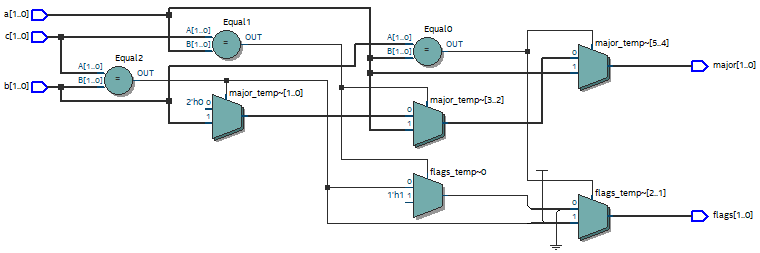
\includegraphics[width=\linewidth]{lab3_4_rtl}
	\caption{Результат синтеза в RLT Viewer}
	\label{fig:lab3_4_rtl}
\end{center}
\end{figure}

\section{Результаты моделирования}
\label{sec:lab3_4_modeling}

На рис. \ref{fig:lab3_4_modeling} изображена временная диаграмма работы синтезированного устройства. На вход устройства поочередно подаются случайные значения \code{a[1:0]}, \code{b[1:0]} и \code{c[1:0]}, признаки достоверности записываются в \code{flags[1:0]}, а мажоритарное значение (если значения хотя бы двух входов одинаковы) в \code{major[1:0]}.

\begin{figure}[H]
\begin{center}
	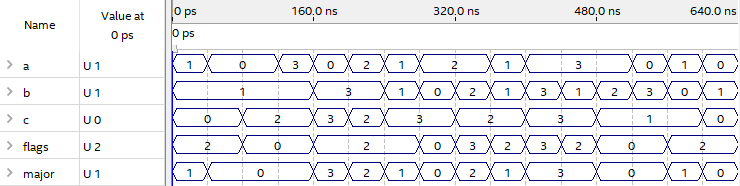
\includegraphics[width=\linewidth]{lab3_4_modeling}
	\caption{Результаты моделирования}
	\label{fig:lab3_4_modeling}
\end{center}
\end{figure}

\section{Назначение выводов СБИС}

На рис. \ref{fig:lab3_4_pins} приведены назначения выводов СБИС в Pin Planner.

\begin{figure}[H]
\begin{center}
	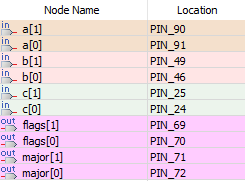
\includegraphics{lab3_4_pins}
	\caption{Таблица назначений в Pin Planer}
	\label{fig:lab3_4_pins}
\end{center}
\end{figure}

\section{Результаты проверки на плате}

Для тестирования проекта на плате были использованы тесты, описанные в пункте \ref{sec:lab3_4_modeling}. Результаты тестирования совпадают с ожидаемыми, следовательно, устройство работает верно.

\section{Выводы}

Реализовано мажоритарное устройство с тремя 2-х разрядными входами. Результаты моделирования и тестирования на плате показали, что разработанное устройство работает верно.
\end{document}